\documentclass{article}
\usepackage{amsmath}
\usepackage{amssymb}
\usepackage{tikz}
\usetikzlibrary{arrows}

\begin{document}

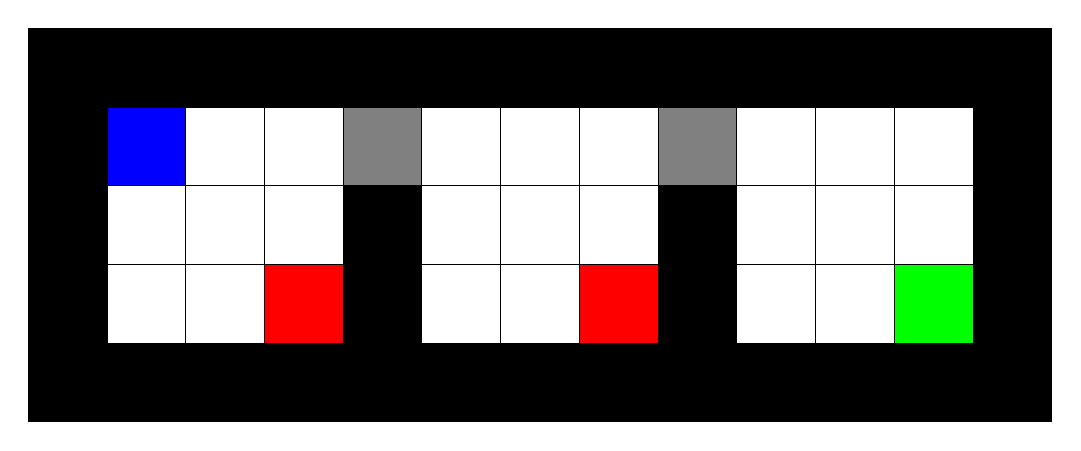
\begin{tikzpicture}
    \def\letterlist{{"black", "black", "black", "black", "black", "black", "black", "black", "black", "black", "black", "black", "black", "blue", "white", "white", "gray", "white", "white", "white", "gray", "white", "white", "white", "black", "white", "white", "white", "black", "white", "white", "white", "black", "white", "white", "white", "black", "white", "white", "red", "black", "white", "white", "red", "black", "white", "white", "green", "black", "black", "black", "black", "black", "black", "black", "black", "black", "black", "black", "black", "black"}}

    \foreach \x in {0,...,12} {
        \foreach \y in {0,...,-4} {
            \pgfmathtruncatemacro{\index}{\x-12*\y}
            \pgfmathsetmacro{\cellContent}{\letterlist[\index]}

            \filldraw[fill=\cellContent, draw=black] (\x, \y) rectangle ++(1, 1);


        }
    }
\end{tikzpicture}

\end{document}